\documentclass[xcolor={usenames,dvipsnames,svgnames}, compress]{beamer}

% \usepackage[utf8]{inputenc}
\usepackage{booktabs}
\usepackage{dcolumn}
\usepackage{colortbl}

% \usepackage[style=authoryear-comp, backref=true]{biblatex}
\usepackage{ifxetex}
\usepackage{amsmath}
\usepackage{biblatex}
% 
\usepackage[no-math]{fontspec}

% 
% CLIPS listings
%\usepackage[utf8]{inputenc}
\usepackage{listings}
\usepackage{xcolor}


%
% I asked on stackoverflow for rainbow parentheses
% http://tex.stackexchange.com/questions/235740/rainbow-parentheses-in-lisp-listings
% the palette is from solarized theme
\definecolor{solarized-cyan}{RGB}{42, 161, 152}
\definecolor{solarized-magenta}{RGB}{211, 54, 130}
\definecolor{solarized-yellow}{RGB}{181, 137, 0}
\definecolor{solarized-violet}{RGB}{108, 113, 196}
\definecolor{solarized-red}{RGB}{220, 50, 47}
\definecolor{solarized-orange}{RGB}{203, 75, 22}
\definecolor{solarized-grey}{RGB}{101, 123, 131}

\lstdefinelanguage{clips}
{
  classoffset=0,
  morekeywords ={deffunction, deftemplate, defglobal, defmodule, defrule, deffacts, nil, assert, retract},
  keywordstyle=\bfseries\color{solarized-orange},
  classoffset=1,
  morekeywords ={delcare, salience, run, slot, multislot, clear, reset, facts, exit, agenda, initial-fact, watch, ppdefrule, unwatch, printout, if, then, else, while, loop-count, crlf, read, readline},
  keywordstyle=\bfseries,
  %classoffset=2,
  %keywordsprefix=\?,
  %alsoletter=\?,
  %keywordstyle=\itshape\color{solarized-red},
  classoffset=0,
  sensitive=true,
  morecomment=[l]{;},
  morestring=[b]{"},
  stringstyle=\color{solarized-grey},
  basicstyle=\scriptsize,%\ttfamily\scriptsize,
  numbers=left,
  numbersep=-5pt,
  numberstyle=\tiny,
  showstringspaces=false,
  }

\renewcommand{\ttdefault}{pcr}

% egreg's modulo macro (see http://tex.stackexchange.com/a/34449/21891)
\def\truncdiv#1#2{((#1-(#2-1)/2)/#2)}
\def\moduloop#1#2{(#1-\truncdiv{#1}{#2}*#2)}
\def\modulo#1#2{\number\numexpr\moduloop{#1}{#2}\relax}    

\makeatletter

% a TeX counter to keep track of the nesting level
\newcount\netParensCount@clisp

% Modify how ( and ) get typeset depending on the value of the counter
% (Based on Ulrike Fischer's approach to modifying characters in listings;
% see http://tex.stackexchange.com/a/231927/21891)
\lst@CCPutMacro
\lst@ProcessOther{`(}{{%
    \ifnum\lst@mode=\lst@Pmode\relax%
    \rainbow@clisp{(}%
    \global\advance\netParensCount@clisp by \@ne%
    \else
    (%
    \fi
  }}%
\lst@ProcessOther{`)}{{%
    \ifnum\lst@mode=\lst@Pmode\relax%
    \global\advance\netParensCount@clisp by \m@ne%
    \rainbow@clisp{)}%
    \else
    )%
    \fi
  }}%
\@empty\z@\@empty
% Color its argument based on the value of the \netParensCount@clisp counter
% (modulo 5)
\newcommand\rainbow@clisp[1]{%
  \ifcase\modulo\netParensCount@clisp 5\relax%
  \textcolor{solarized-cyan}{\bfseries#1}%
  \or
  \textcolor{solarized-yellow}{\bfseries#1}%
  \or
  \textcolor{solarized-magenta}{\bfseries#1}%
  \or
  \textcolor{solarized-violet}{\bfseries#1}%
  \else
  \textcolor{solarized-red}{\bfseries#1}%
  \fi
}

% Alternatively, you could simplify the definition of \rainbow@clisp to...
% \newcommand\rainbow@clisp[1]{%
% \textcolor{color\modulo\netParensCount@clisp 5}{#1}%
% }
%   ... but this assumes that the colours have names of the form color<i>,
%   where <i> is a positive integer

%   reset the counter at the beginning of each listing
%   (just in case there were unmatched parentheses in a previous listing)
\lst@AddToHook{PreInit}{%
  \global\netParensCount@clisp 0\relax%
}

\makeatother




\lstnewenvironment{clips-code}[1][]
{\lstset{language=clips,
    #1
  }}
{}






%%% Local Variables:
%%% mode: latex
%%% TeX-master: t
%%% End:


\definecolor{jess-fucsia}{RGB}{170, 0, 127}


\hypersetup{
  colorlinks=true,       % false: boxed links; true: colored links
  linkcolor=jess-fucsia,          % color of internal links (change box color with linkbordercolor)
  % citecolor=green,        % color of links to bibliography
  %filecolor=magenta,      % color of file links
  urlcolor=jess-fucsia           % color of external links
}

%%% Local Variables:
%%% mode: latex
%%% TeX-master: t
%%% End:




\usepackage{lacamlisciotheme/beamerthemelacamliscio}

% \lstdefinelanguage{java}
% {
%   classoffset=0,
%   morekeywords ={deffunction, deftemplate, defglobal, defmodule, defrule, deffacts, nil, assert, retract},
%   keywordstyle=\bfseries\color{solarized-orange},
%   classoffset=1,
%   morekeywords ={delcare, salience, run, slot, multislot, clear, reset, facts, exit, agenda, initial-fact, watch, ppdefrule, unwatch, printout, if, then, else, while, loop-count, crlf, read, readline},
%   keywordstyle=\bfseries,
%   % classoffset=2,
%   % keywordsprefix=\?,
%   % alsoletter=\?,
%   % keywordstyle=\itshape\color{solarized-red},
%   classoffset=0,
%   sensitive=true,
%   morecomment=[l]{;},
%   morestring=[b]{"},
%   stringstyle=\color{solarized-grey},
%   basicstyle=\scriptsize,%\ttfamily\scriptsize,
%   numbers=left,
%   numbersep=-5pt,
%   numberstyle=\tiny,
%   showstringspaces=false,
% }
\lstnewenvironment{java-code}[1][]
{\lstset{language=java,
    #1
  }}
{}

% 
% customizing itemize items
% \setbeamertemplate{itemize item}{\textbf{\unichar{"2295}}}
% \setbeamertemplate{itemize item}{\raise .4ex\hbox{\tiny\textcolor{lacamlilac}{$\boldsymbol{\oplus}$}}\hspace{-2pt}}
% \setbeamertemplate{itemize subitem}{\raise .2ex\hbox{\tiny\textcolor{lacamlilac}{$\boldsymbol{\otimes}$}}\hspace{-2pt}}
% \setbeamertemplate{itemize subsubitem}{\textcolor{lacamlilac}{$\oplus$}}
% \setbeamertemplate{bibliography item}{\hspace{10pt}\raise .2ex\hbox{\tiny\textcolor{lacamlilac}{$\boldsymbol{\oplus}$}}}


% \addbibresource{../referomnia/referomnia.bib}

\setbeamertemplate{headline}{}

%%%%%%%%%%%%%%%%%%%%%%%%%%%%%%%%%%%%%%%%%%%%%%%%%%%%%%%%%%%% 
%%%%%%%%%%%%%%%%%%%%%%%%%%%%%%%%%%%%%%%%%%%%%%%%%%%%%%%%%%%% 
%%%%%%%%%%%%%%%%%%%%%%%%%%%%%%%%%%%%%%%%%%%%%%%%%%%%%%%%%%%% 


\begin{document}

% \title{Metodi di Apprendimento Statistico-Relazionale: Sum-Product Network \& Co-clustering}
\title{Embedding CLIPS}
%\subtitle{An Introduction}
\author{Antonio Vergari}
% \institute{Lacam$@$DIB$@$Uniba}
\institute{Università degli Studi di Bari}
\department{Dipartimento di Informatica}
\laboratory{LACAM}
\group{Machine Learning}
\institutelogo{
\includegraphics[width=25pt]{Figures/unibaba}}
\lablogo{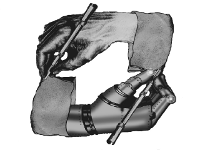
\includegraphics[width=35pt]{Figures/lacam}}

\footnotesize \let\small\footnotesize





{
  \setbeamertemplate{headline}{}
  \setbeamertemplate{footline}{}
  \begin{frame}
    \titlepage
  \end{frame}
}






\section{Embedding CLIPS in Java}
{\setbeamertemplate{headline}{}
  \begin{frame}
    \sectionpage
  \end{frame}
}

\begin{frame}
  \frametitle{CLIPSJNI}
  To host CLIPS from Java code one can use\footnote{Alternatives like
    Jess allow foreign languages to communicate both directions.} the
  \href{http://clipsrules.sourceforge.net/CLIPSJNIBeta.html}{\textsf{CLIPS
      Java Native Interface}}, whose latest version is beta
  0.4.\par\bigskip

  In order to properly install it one has to make sure to have:
  \begin{itemize}
  \item the compiled library (which is a \textsf{.dll} file under Windows, \textsf{.so}
    for Linux, and \textsf{.jnilib} for OS X)
    \item the proper CLIPSJNI.jar file containing the lib headers,
      sources and a compiled version of the interpreter
  \end{itemize}\bigskip

  To correctly write and run a Java program calling CLIPS routines,
  you have to:
  \begin{itemize}
  \item compile the code by putting in the classpath the CLIPSJNI.jar
    file
    \item run the compiled classes by putting again the CLIPSJNI.jar
      in the classpath and specifying the library path through the
      attribute \textsf{java.library.path}.
  \end{itemize}
\end{frame}

\begin{frame}[fragile]
  \frametitle{CLIPS JNI library}
  With the downloaded version come the pre-compiled binaries for OS X
  (\textsf{libCLIPSJNI.jnilib}) and for 32 and 64-bit version of
  Windows (\textsf{CLIPSJNI32.dll} \textsf{CLIPSJNI64.dll}). For
  linux users one has to compile it by itself (sigh). To do so: enter
  the \textsf{library-src} folder and execute\footnote{
     For different
     Linux distros one can experience different errors during compilation,
     please follow
     \href{https://pimpmylinux.wordpress.com/2011/05/24/compilare-clipsjni-su-linux-32-e-64-bit/}{this
       link}
     for common problem solving like setting
    the \textsf{JAVA\_HOME} system var or the flags under  64 bits distributions
  }
  \begin{clips-code}
    make -f makefile.linux
  \end{clips-code}\par\bigskip
  Save the library under a meaningful path and remember it. Optionally
  one can specify it globally by putting it under Java lib dir.
  
\end{frame}

\begin{frame}[fragile]
  \frametitle{A simple sample project I}
  CLIPS framework can be accessed through one (or more) instance(s) of
  the object \textsf{Environment}. The callable methods of the object
  are the ways to access CLIPS interactive commands. Their names are
  self explanatory: \textsf{clear}, \textsf{reset},
  \textsf{assertString}, \textsf{eval},\dots\par

  Now suppose our first Java program shall be a little REPL that takes
  a command from the console stdin, evaluates it by calling CLIPS
  \textsf{eval} functions and prints back to the console stdout the
  result.\par

  
  \begin{java-code}
    import CLIPSJNI.*; // importing APIs

    public class ClipsREPL {
      Environment clips = null; // Declaring an environment
      ClipsREPL() {
        clips = new Environment(); /* Instantiating a new environment */
        clips.clear(); /* clearing it */
      }
      ...
    }
  \end{java-code}
  
\end{frame}

\begin{frame}[fragile]
  \frametitle{A simple sample project II}
  The main method implementing the REPL:
  \begin{java-code}
    void repl() {
      boolean endInteraction = false;
      Scanner in = new Scanner(System.in);
      while(!endInteraction) {
        System.out.print("CLIPS> ");
        String userInput = in.nextLine(); /* Read */
        try {
          String response = clips.eval(userInput).toString(); /* Eval */
          System.out.println(response); /* Print */
          if(response.equals("(exit)")){ /* Loop */
             endInteraction = true;}
        }catch(Exception e) {
          e.printStackTrace();}}}
  \end{java-code}

  Mind the use of the \textsf{eval} method of \textsf{Environment}, it
  throws a generic \textsf{Exception} (sigh). Potentially, you can call
  every CLIPS interactive command with that.
\end{frame}

\begin{frame}[fragile]
  \frametitle{A simple sample project III}
  To compile our \textsf{.java} file in a \textsf{.class}, we have to
  specify where the \textsf{CLIPSJNI.jar} has been saved:
  \begin{clips-code}[numbers=none]
    javac -classpath <path-to-CLIPSJNI.jar> ClipsREPL.java
  \end{clips-code}\bigskip

  To execute it, we need to specify a complete path\footnote{Remind to
  include all the needed path with \textsf{-cp}, even the current one
  if necessary. Path concatenation is done with ``;'' under UNIX and
  ``:'' on Windows.}
  \begin{clips-code}
    java -cp .;<path-to-CLIPSJNI.jar> -Djava.library.path=<path-to-CLIPSJNI-lib> ClipsREPL
  \end{clips-code}\bigskip

  Have a look at the other included examples to see other uses.
\end{frame}

\begin{frame}[fragile]
  \frametitle{A simple diagnostic classifier revised}
  Write a small Java program embedding a shorter version of the simple
  classifier to diagnose icterus diseases.\par
  \begin{java-code}
    clips.load("icterus-simple.clp");
  \end{java-code}
  This time there are no
  rules prompting the user for observed symptoms, you have to gather
  them from Java (from the command line, for instance, or even from a
  GUI).\par\bigskip
  After you properly ask the user what the symptoms are, you have to
  assert in the WM the corresponding facts. \textbf{Hint:} use the assertString
  function of the Environment.\par\bigskip

  To apply inference you can simply call the Environment method
  \textsf{run}.\par\bigskip

  Instead, to retrieve a fact, for instance to check whether a
  diagnosis has been asserted, you can call the CLIPS defined function 
  \begin{java-code}
    PrimitiveValue fv =
        clips.eval("(get-all-facts-by-names diagnosis)").get(0);
    String diagnosis = fv.getFactSlot("name").toString();
  \end{java-code}
\end{frame}


\end{document}


%%% Local Variables:
%%% mode: latex
%%% TeX-engine: xetex
%%% TeX-master: t
%%% End:
